
\setvruler[][][][3][0]
\chapter{Introduction}
\pagenumbering{arabic}
\setcounter{page}{1}

This document specifies a collection of compiler
directives, i.e., runtime library routines that can be used to specify
distributed-memory parallel programming in \C and \Fort
programs. These compiler directives define the specifications of the \XMP Application
Program Interface (\XMP API). These specifications provide a
model of parallel programming for distributed memory multiprocessor
systems. The directives extend the \C and \Fort base languages to
describe distributed memory parallel programs.

\section{Scope}

\XMP API
is used to explicitly specify the action to be taken by the compiler
and the runtime system to execute the parallel program in a distributed
memory system. \XMP-compliant implementations are not required
to check for invalid local data access, data conflicts, racing
conditions, or deadlock. The \XMP is defined by following items:

\begin{itemize}
\item A set of directives
\item Minimum language extension on base languages (\C and \Fort)
\item Runtime libraries
\item Environment Variables
\end{itemize}

\section{Features of \XMP}

The features of \XMP are summarized as follows:

\begin{description}
\item {\bf Language extensions} for familiar languages, such as \C and FORTRAN,
  that can reduce code-rewriting and educational costs.
\item \XMP supports typical parallelization based on the {\bf data parallel
  paradigm} and work sharing under {\it global view} and enables
  parallelization of the original sequential code with minimal
  modification using simple {\bf directives}, such as \OMP. 
\item \XMP also includes a CAF-like Partitioned
Global Address Space (PGAS) feature as {\it local-view} programming. 
\item {\bf Explicit communication and synchronization}. All actions
  are taken by directives for being ``easy-to-understand'' for
  performance-aware programming 
\item For flexibility and extensibility, the execution model
allows {\bf combination with explicit \MPI coding} for more complicated
and tuned parallel codes and libraries. 
\item For multi-core and SMP clusters,
{\bf \OMP directives can be combined} into \XMP for thread
programming inside each node as a hybrid programming
model.
\end{description}

\XMP is being designed based on experience obtained in the development of HPF, Fujitsu XPF
(VPP FORTRAN), and OpenMPD.  

\chapter{Overview of the \XMP model and language}

\section{Hardware model and execution model}

The target of \XMP is a distributed memory system
(Figure \ref{fig1}). Each computation node, which may have
several cores sharing main 
memory, has its own local memory, and each node is connected via
network. Each node can access and modify its local memory directly
and can access the memory on other nodes via communication. However, it is assumed that accessing remote memory is much slower than
accessing local memory.

The basic execution model of
\XMP is a Single Program Multiple Data (SPMD) model on
distributed memory. In each node, a program starts from the same main
routine. An \XMP program begins as a single thread of execution
in each node. 

When the thread encounters \XMP directives,
synchronization and communication occurs between nodes. In other words,
no synchronization or communications occur without directives. In
this case, the program performs duplicate execution of the same program
on local memory in each node.

\OMP API can be used in order to
make use of multicores in a node. In this specification, we define
actions only when \XMP directives are executed one thread at a time .

\begin{myfigure}
\includegraphics[width=12cm]{figs/Fig1.eps}
  \caption{Hardware Model}\label{fig1}
\end{myfigure}

By default, data declared in the program are allocated in each node and are referenced
locally by threads executed in the node. 

\XMP supports two models of data viewing: the global-view programming model and the local-view programming model. In the local-view programming model, accesses to data
in remote nodes is performed explicitly by language extension for get/put
operations on remote nodes with the node number of the target nodes, while
reference to local data is executed implicitly. 

In contrast to
a local-view programming model, a global-view programming model is
a model in which programmers express their algorithm and data structure in their entirety, mapping them to the node set. The programmers describe the
data distribution and the work mapping in order to express how to distribute
data and share the workload among nodes. The variables in the global-view
programming model appear as a shared memory spanning the nodes.

\section{Global-view programming model}

The global-view
programming model is useful when, starting from sequential version of
the program, the programmer parallelizes the program in the data-parallel model by
adding directives incrementally with minimum modification. In the
global-view programming model, the programmer describes the data
distribution of the data shared among the nodes by data distribution
directives. {\tt loop} iteratively construct maps to the node where the 
computed data is located. Global-view communication directives are
used for synchronization between nodes, to maintain the consistency of the shadow
area, and to move part of the distributed data globally. Note 
that the programmer must perform all computations
that require data reference locally by any appropriate directives. 

In many cases, the
\XMP program using the global-view programming model is based on a sequential
program and can produce the same results independent of the
number of computation nodes (Figure \ref{fig2}). The
global view provides a 
programming model in which computation and data are distributed onto
computation nodes.

There are three groups of directives for the
global-view programming model. Since these directives can be ignored as a
comment by the compilers of base languages (\C and \Fort), an
\XMP program derived from a sequential program can preserve the
integrity of the original program when the program is run sequentially. 

\subsubsection*{Data Mapping}
Specify the data distribution and mapping to nodes (partially
inherited from HPF).

\subsubsection*{Work Mapping (Parallelization)}
Assign tasks to nodes. The {\tt loop} construct maps each iteration to
nodes containing the referenced elements, and the Task construct
executes each task in parallel in different node sets.

\subsubsection*{Communication and Synchronization}
Describe how to communicate and synchronize with the other compute
nodes. In \XMP, inter-node communication must be described
explicitly. The compiler guarantees that communication takes place
only if communication is explicitly specified.

\begin{myfigure}
\includegraphics[width=12cm]{figs/Fig2.eps}
  \caption{Parallelization by the global-view programming model}
\label{fig2}
\end{myfigure}

\section{Local-view programming model}

The local-view programming model is suitable for 
programs that explicitly describe the algorithm of each node and for explicit
remote data reference (Figure \ref{fig3}). Since MPI is
considered to have a local view, the local-view programming model of \XMP has high
interoperability with MPI.

For the local-view programming model,
the language extension and some directives are provided. The coarray
notation taken from \CAF (CAF) is such an extension. For
example, in order to access an array element of {\tt A(i)} located on compute
node {\tt N},
the expression of {\tt A(i)[N]} is used. If the access is a value reference,
then communication to obtain the value occurs. If the access is to 
update the value, then communication to set a new value occurs.

\begin{myfigure}
\includegraphics[width=12cm]{figs/Fig3.eps}
  \caption{Local-view programming model}
\label{fig3}
\end{myfigure}

\section{Interactions between global view and local view}

The node in
\XMP is used to distribute data or the computational
load. In the local view, the node is used in conjunction with the coarray
directive to reference data. In the application program, programmers
should choose an appropriate data model according to the structure of
the program. Figure \ref{fig4} illustrates the global view and the local view of data.

Data may have a global view and local view and can be
accessed from either view. \XMP provides some
directives to set the local name (alias) to the global data declared in
the global-view programming mode so that the data can also be referenced 
in the local-view programming model. It may be useful to optimize the
program by explicit remote data reference in the local-view programming model.


\begin{myfigure}
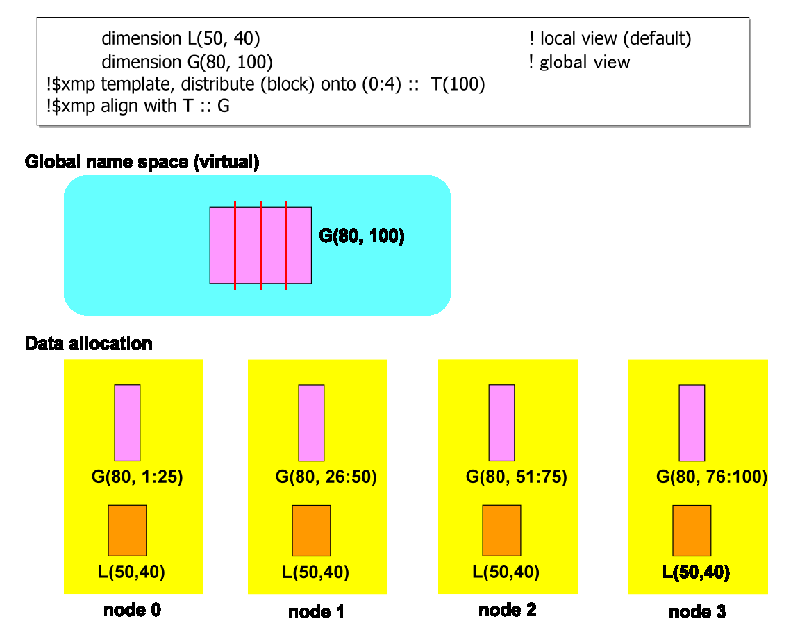
\includegraphics[width=12cm]{figs/Fig4.eps}
  \caption{Global view and local view}
\label{fig4}
\end{myfigure}

\section{Execution model and task}


In \XMP, a program begins as a single thread
of execution in each node. The set of nodes when starting a program is
referred to as the entire node set.

A task is a specific instance of executable
code and its data environment executed in a set of nodes. A task when
starting a program in the entire node set is called an initial task. The
initial task can generate a subtask, which is executed on a subset of the
nodes by the {\tt task} construct. A set of nodes executing the same task is
referred to as the set of executing nodes. If no {\tt task} construct is encountered, then a
program is executed as a single task, and its executing nodes are the entire node set.

If no directives are encountered, then a program is executed
locally. When the same codes are executed, almost the same computation is
performed in each node, which is referred to as duplicate execution. When the threads
encounter a {\tt loop} construct or an {\tt array} construct, the specified
loop is executed in parallel, so that each iteration is assigned to the
node where the specified data element is located. 

A new task is generated by
the {\tt task} construct. A code in the {\tt task} construct is executed
as a subtask executed in a specified node set. When a subroutine is
called in the context of the task, the subroutine is executed on its
executing nodes. 

For synchronization and communication between nodes, a set of
directives is provided. In the local-view programming model, coarray
features are adopted for remote data reference. Note 
that all synchronization and communication are specified explicitly by directives, and without such directives, no communications are
executed implicitly by the compiler.
